\chapter{Хранение и передача данных}

Сохранять и считывать данные несложно. Например, можно записать единички
и нолики на бумаге и прочитать, когда потребуется вспомнить эту последовательность.

Но для автоматического устройства, которое мы хотим создать, бумага и ручка подходят плохо.
Можно <<записать>> единички и нолики, набрав их на тумблерах.
<<Считать>> сохранённую в их положениях информацию можно подключив тумблеры к электрической цепи:
например, зажечь лампочки или даже отправить запомненные символы электронным письмом.

Но кто будет переключать все эти тумблеры? Хотелось бы, чтобы при появлении сигнала во входной цепи,
его можно было запомнить без участия человека (операция записи),
а затем, через произвольное время, когда входной сигнал уже пропал,
получить такой же сигнал в выходной цепи (операция чтения).

То, что нам нужно, называется ячейкой памяти. Ячейки могут отличаться объёмом хранимой информации,
способами управления и элементной базой. Сейчас мы рассмотрим такую ячейку, построенную на электромагнитных реле.


\section{RS-триггер}

Хранение одного бита можно сделать с помощью одного реле.
Если оно включается с помощью внешнего сигнала, то реле <<сохраняет>> единицу.
Но когда внешний сигнал пропадает, сохранённая единица пропадает тоже,
потому что на катушке реле больше нет напряжения.

Чтобы включённое состояние запоминалось, нужно организовать обратную
связь через один из контактов реле. Как только реле включается с помощью
входа $SET$, на его
обмотку подаётся напряжение через его же замкнутый контакт. Поэтому даже
если перестать подавать напряжение на вход $SET$, реле всё равно останется включённым:

\begin{center}
\includegraphics{schemes/trigger1.png}
\end{center}

Но если такое реле уже включилось, выключить его не получится. Единственный способ~---
это отключить питание всей схемы. Тогда контакты разомкнутся и при повторной подаче питания реле будет
в выключенном состоянии.

Чтобы не отключать всю схему, нужно предусмотреть отдельное реле, позволяющее
отключить питание только для запоминающего реле:

\begin{center}
\includegraphics{schemes/trigger2.png}
\end{center}

Теперь подав сигнал на вход $RESET$, можно выключить реле, которое <<запомнило>> единицу.
И на его выходе опять окажется ноль.

Устройство (ячейка памяти) для хранения одного бита информации называется триггером.
Чтобы его сделать нам потребовалось два реле, но когда мы
говорим о состоянии триггера, то речь идёт о том, включено или выключено то самое
<<запоминающее>> реле.
Например, если оно включено, то в триггере хранится единица.

Триггер с двумя входами $RESET$ и $SET$ называется RS-триггером.
На практике удобно объединить несколько таких триггеров в многобитовый регистр
и использовать для них единый сигнал сброса, сэкономив несколько реле:

\begin{center}
\includegraphics{schemes/trigger3.png}
\end{center}

\section{Шина}

Шина --- это набор проводников, объединённых общим назначением.
К этим проводникам подключаются несколько устройств для обмена сигналами.

Например, к внутренним шинам компьютера могут быть подключены память и
жёсткий диск. Тогда по шине данных передаются данные между процессором и памятью
или процессором и жёстким диском, шина адреса используется для выбора определённой
ячейки в памяти, а по шине управления приходят сигналы,
позволяющие отличать обращение к памяти от обращения к диску.

Так как к шине обычно подключается больше двух устройств,
необходимо изолировать те из них, которые не участвуют в обмене данными
в конкретный момент времени.
Например, когда процессор взаимодействует с памятью через шины
данных или адреса, жёсткий диск не должен подключаться к тем же шинами.
В противном случае сигналы получатся некорректными, а может одно из устройств даже сгорит.

В релейном компьютере мы можем использовать для подключения к четырёхбитной шине
шинный формирователь из одного реле:

\begin{center}
\includegraphics{schemes/bus.png}
\end{center}

Когда реле включается, оно соединяет подключённое к нему устройство с шиной.
Таким устройством может быть набор из нескольких триггеров (позднее мы будем называть его регистром).
Подключение будет двунаправленным, поэтому с помощью этой схемы можно как
записывать данные в регистр, так и считывать оттуда.

Таким образом, сигнал $SELECT$ подаётся на шинные формирователи только тех устройств,
которые должны повзаимодействовать через шину. Остальные устройства, подключённые
к шине, остаются изолированными от неё.

% \section{Шины в конструкторе}

% В конструкторе все модули могут подключаться к шинам по которым передаются от~$1$ до~$4$ сигналов.

% Например, $4$ сигнала могут использоваться для управления модулем регистра.
% Или для передачи данных из одного регистра в другой.
% Каждым из таких сигналов можно управлять с помощью модуля переключателей,
% соединив его с соответствующим разъёмом регистрового модуля.

% Иногда соединения двух модулей напрямую невозможны, потому что модули приходится
% расположить не рядом. Тогда нужно использовать проводные шлейфы, присоединяемые
% к соответствующим разъёмам.

\section{Регистр}

Регистры внутри процессоров (или периферийных устройств)
используются для хранения данных и для проведения вычислений.
Регистры могут иметь выделенное назначение (например, хранить режим работы устройства
или счётчик инструкций), а могут быть универсальными
(в разные моменты хранить адреса, операнды арифметических операций,
значения для ввода-вывода).

На схеме регистрового модуля можно увидеть $8$ реле:

\begin{center}

\includegraphics[width=\columnwidth]{schemes_components/register.png}
\end{center}

% Четыре из них это реле для хранения данных,
% ещё одно реле нужно для обнуления регистра (оно расположено на схеме слева)
% а три оставшиеся используются для подключения к шинам данных (эти реле справа).

Для хранения данных используются RS-триггеры, описанные выше,
но сигнал для сброса у них общий. Таким образом, записывать
данные можно только во все четыре бита сразу. Поэтому такой
модуль и реализует функции цельного регистра, а не нескольких
разрозненных RS-триггеров.

Также модуль регистра содержит три шинных формирователя.
Их можно использовать для подключения триггеров к разным устройствам
через три шины. Например, одна шина может быть предназначена
для первого операнда при вычислениях, вторая для второго операнда,
а третья для копирования данных между регистрами.

Выглядит плата регистрового модуля так:

\begin{center}
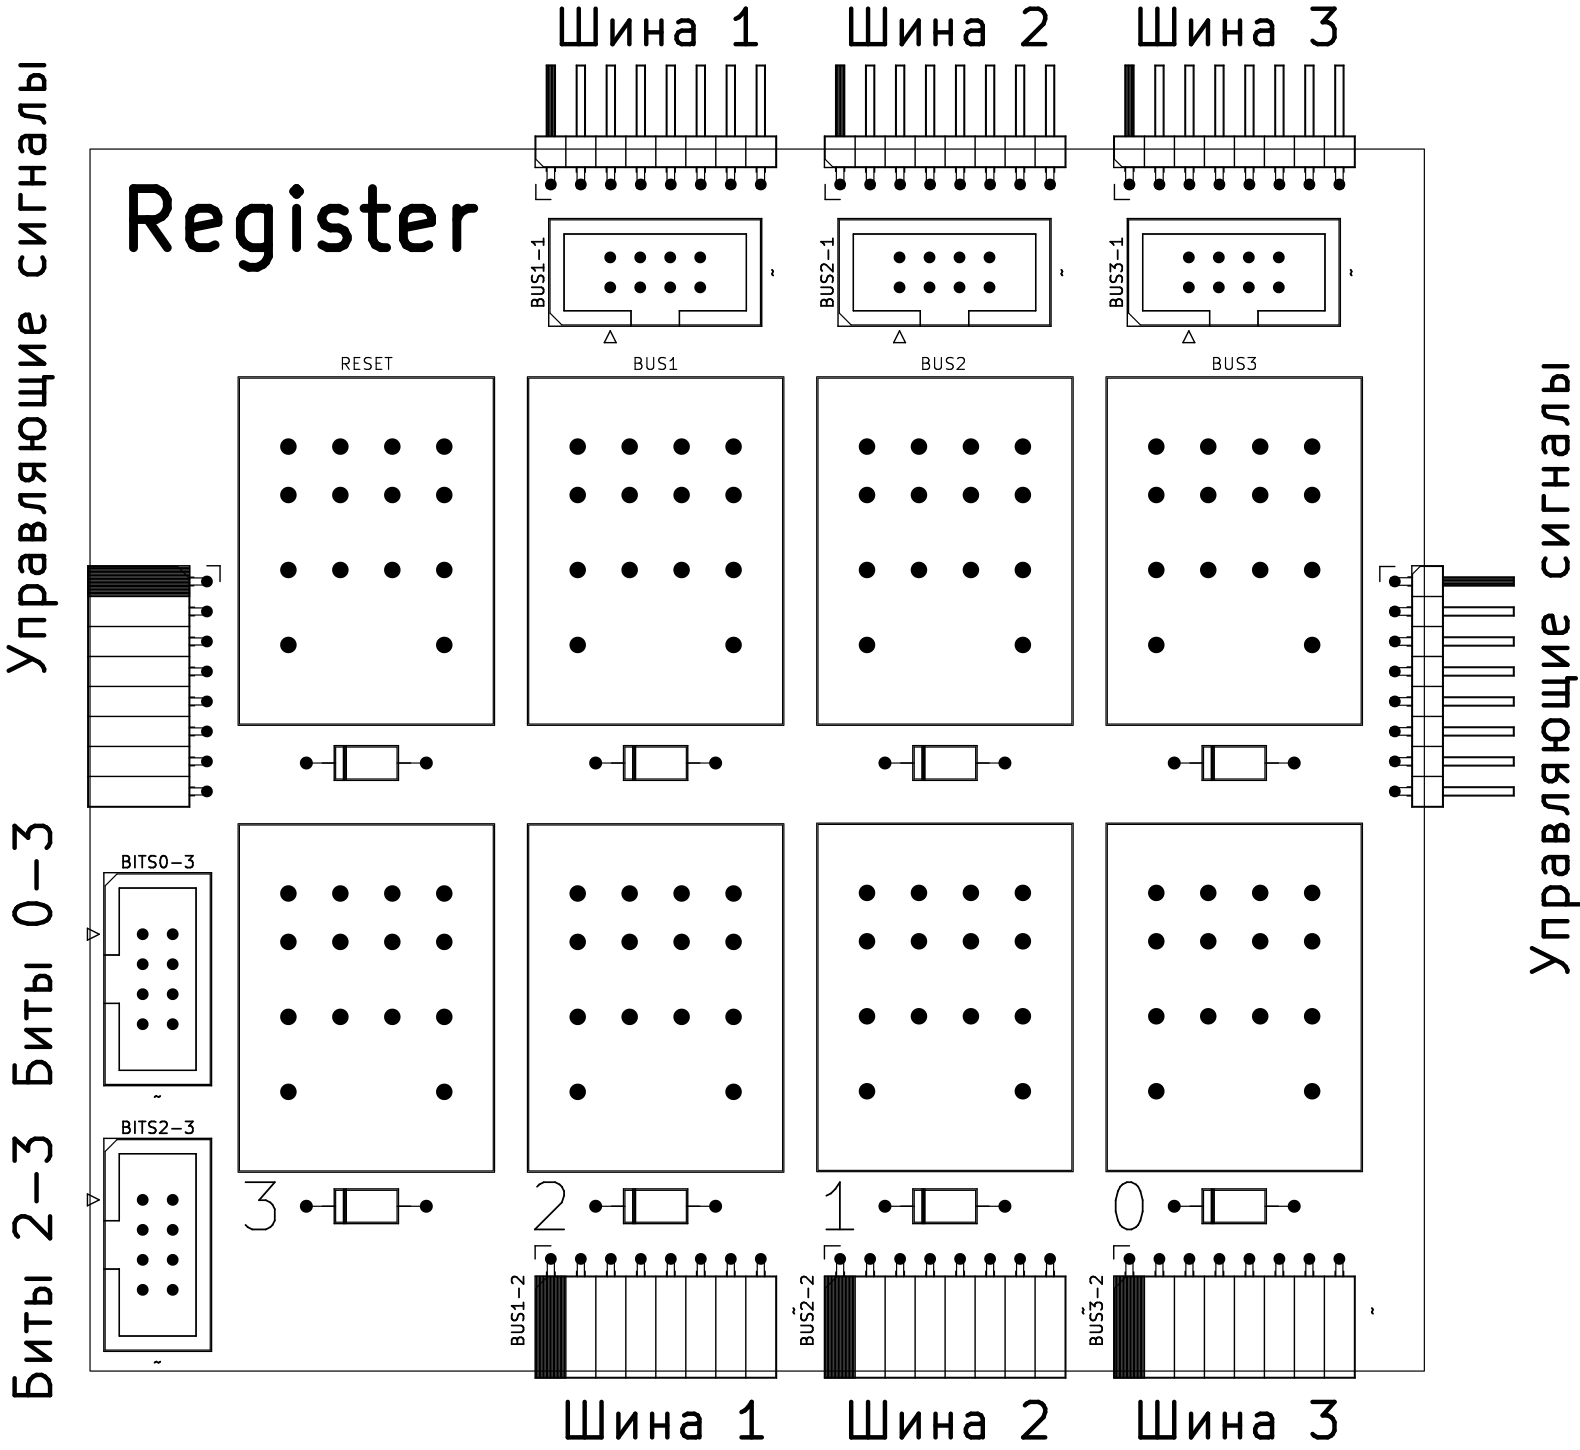
\includegraphics{boards/register.png}
\end{center}

Если на плату регистра установить только реле шинных формирователей,
получится модуль, который может подключать четырёхбитные сигналы
(полученные из разъёма с обозначением $0-3$ для прямого чтения значений триггеров) к одной
из выбранных шин.

На плате регистра есть следующие разъёмы:
\begin{itemize}
  \item Слева и справа: управляющие сигналы сброса и выборки.
        Можно подключить тумблеры
        для ручного включения сигналов. Также можно соединить несколько
        модулей регистра, чтобы управлять одним набором сигналов сразу
        для $8$, $12$ \ldots бит.
  \item Сверху и снизу: три шины данных. Реле регистра могут
        подключаться к шинам для записи или чтения данных.
  \item Разъёмы с битами $0-3$ и $2-3$ для прямого чтения или
        записи триггеров без подключения к шине через шинный формирователь.
\end{itemize}

Чтобы прочитать значение регистра нужно активировать сигнал выборки
его на нужную шину. А уже через шину сигналы поступят на вход какой-то
другой схемы.

Для записи значения в регистр нужно сначала обнулить его триггеры,
иначе запись не произойдёт в тех битах, где уже хранятся единицы.
После этого регистр подключается к нужной шине, и триггеры
защёлкивают нужное значение.


\subsection{Практикум}

\subsubsection{Работа регистрового модуля}


Список модулей:
\begin{itemize}
    \item Модуль переключателей: $2$ штуки
    \item Регистровый модуль: $1$ штука
\end{itemize}

\subsubsection{Регистр без шины}

Сначала соберём схему, в которой не используется соединение регистра и тумблеров
через шинный формирователь, чтобы продемонстрировать, что шина всё-таки нужна.

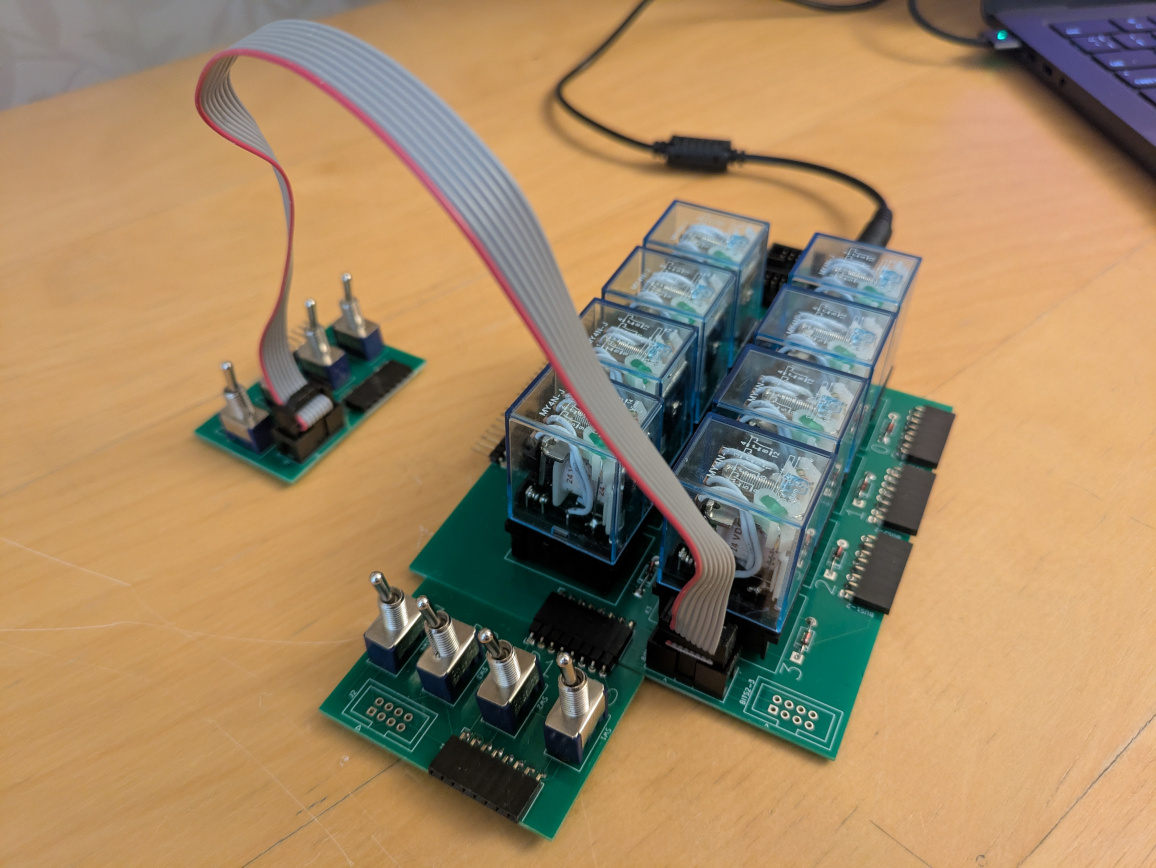
\includegraphics[width=0.5\columnwidth]{photo/register_direct.jpg}


\begin{enumerate}
    \item Подключите тумблеры кабелем (для этого разъёма нет другого варианта) к битам $0-3$ вместо шины.
          Это позволит нам управлять включением триггерных реле непосредственно с помощью тумблеров.
    \item Набирайте значение на тумблерах, подключенных кабелем.
          Убедитесь, что биты переключаются в $1$, но не возвращаются в $0$, если тумблер переключить обратно.
    \item Включите и выключите сигнал сброса (тумблеры, подключенные к боковому разъёму).
          Убедитесь, что для тех тумблеров, что переключены в $1$, соответствующие реле не сбрасываются.
    \item Обнулите тумблеры, управляющие триггерами (те, что подключены проводом).
    \item Включите и выключите сигнал сброса.
          Убедитесь, что значения всех битов теперь $0$.
\end{enumerate}

\subsubsection{Регистр с шиной}

Неудобство первого варианта схемы
в том, что приходится выключать все тумблеры, чтобы можно было просто сбросить все биты регистра.
А ведь это могут быть не тумблеры, а какое-то другое устройство (к примеру, ещё один
регистр), который может быть не согласен сбрасываться.

Поэтому изменим схему следующим образом:

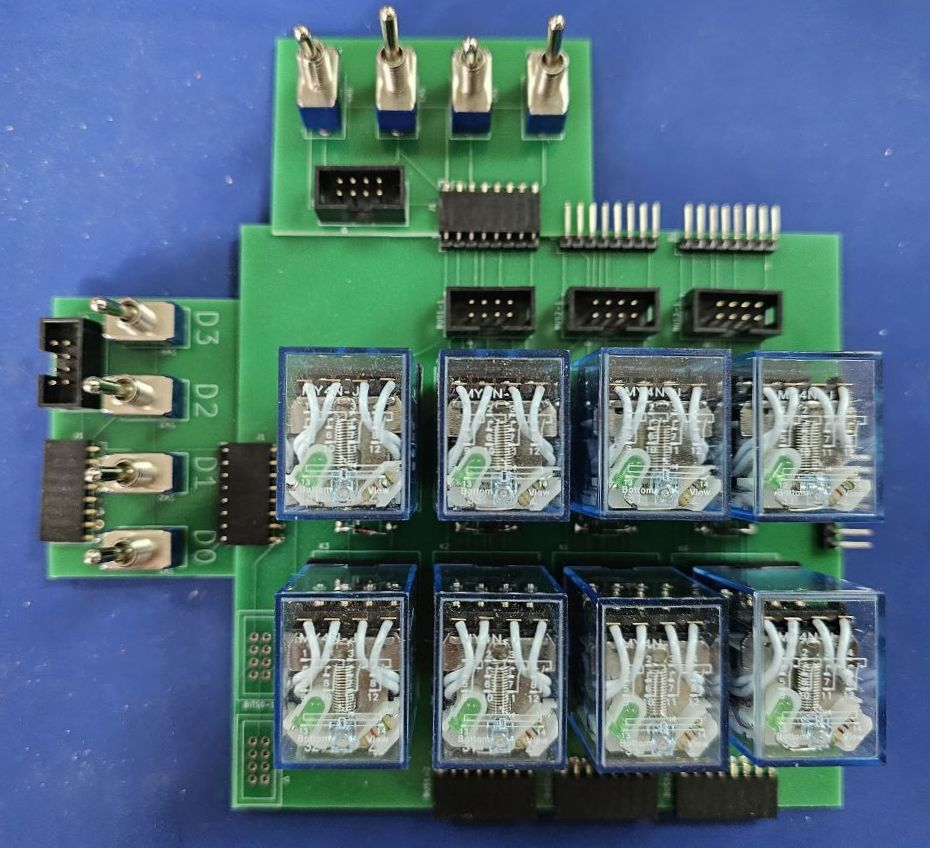
\includegraphics[width=0.5\columnwidth]{photo/register.jpg}

\begin{itemize}
  \item Тумблеры слева управляют работой регистра. Бит~$0$ --- сброс триггеров регистра,
        бит~$1$ --- выборка на шину~$1$.
        Тумблеры~$2$ и $3$ здесь не используются.
  \item Тумблеры сверху нужны для ввода значения регистра. Когда он подключается к шине~$1$,
        значение, набранное на тумблерах, записывается в регистр.
\end{itemize}

Теперь можно проверить, что изменилось в работе схемы:

\begin{enumerate}
    \item Отключите все управляющие сигналы.
    \item Наберите значение на тумблерах для данных. Убедитесь, что это не влияет на регистр.
    \item Включите и выключите сигнал выборки на шину $1$. Убедитесь, что данные записались в регистр.
    \item Включите и выключите сигнал сброса. Убедитесь, что значения всех битов теперь $0$.
          Состояния тумблеров, присоединённых к шине, никак не помешали выполнить сброс.
\end{enumerate}

\subsection{Задачи}

\begin{enumerate}
    \item Возьмите два регистровых модуля и придумайте,
          как скопировать данные из одного регистра в другой, не запоминая их в голове.
\end{enumerate}


\chapter{Хранение больше четырёх бит}

\section{Регистровый файл}

Несколько регистров можно соединить в регистровый файл.
Регистровый файл --- это набор регистров, которые принадлежат одному устройству.
Например, в регистровом файле процессора будет счётчик инструкций,
регистры для хранения арифметических операндов, а также для хранения адреса
при обращении к памяти.

Регистры объединены в регистровый файл, потому что процессор при выполнении операций
делает с регистрами похожие действия. Копирует один в другой, берёт их в разном порядке
для вычислений, записывает в память. Поэтому все регистры должны находиться <<рядом>>,
чтобы схема работы с ними не была слишком сложной.

В нашем конструкторе у каждого из регистров есть сигналы выборки на одну из трёх шин.
Для одного регистра эти сигналы могут активироваться как поочерёдно, так и одновременно
(хотя второе требуется редко).
Если два регистра подключены к одной шине одновременно,
то значения одного копируются в другой. Если точнее,
включённые биты включают аналогичные в другом регистре, то есть
копирование происходит в обе стороны одновременно.

Нулевые биты при этом копироваться не могут. Для записи нулей
регистр необходимо сбросить.


\subsection{Практикум}


Список модулей:
\begin{itemize}
    \item Модуль переключателей: $5$ штук
    \item Регистровый модуль: $4$ штуки
\end{itemize}

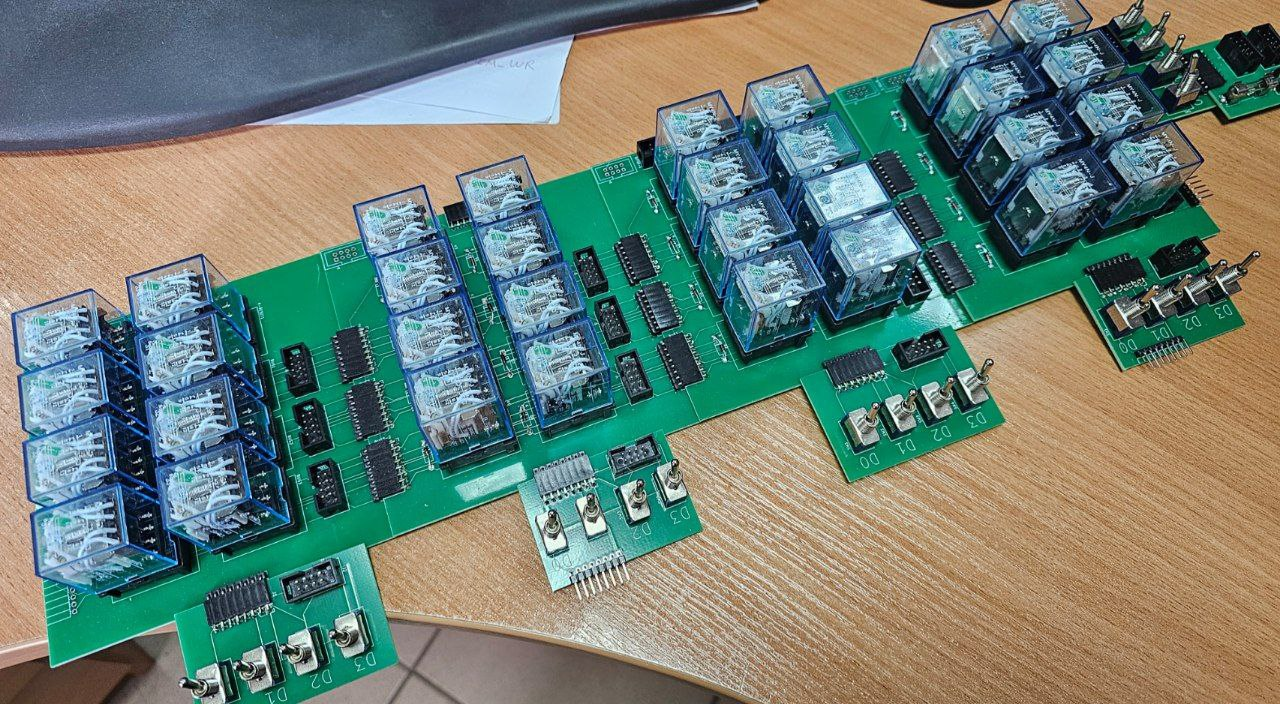
\includegraphics[width=\columnwidth]{photo/register_file.jpg}

Запись в регистры:

\begin{enumerate}
    \item Отключите все управляющие сигналы.
    \item Наберите значение на тумблерах, подключённых к шине данных $1$.
    \item Подключите с помощью тумблера регистр к шине $1$. Убедитесь, что в него записалось набранное значение.
    \item Отключите регистр от шины.
    \item Установите другое положение тумблеров, подключённых к шине данных.
    \item Подключите любой другой регистр к шине $1$. Убедитесь, что в него записалось набранное значение.
\end{enumerate}

Копирование значения:

\begin{enumerate}
    \item Отключите все управляющие сигналы.
    \item Подключите регистр с ненулевыми битами к шине $2$.
    \item Подключите пустой регистр к шине $2$. Убедитесь, что он получил такое же значение, что и в первом регистре.
    \item Отключите все управляющие сигналы.
    \item Аналогично проверьте шину $3$.
\end{enumerate}


\subsection{Задачи}

\begin{enumerate}
    \item Пронумеруйте в уме регистры слева направо или сверху вниз (смотря как у вас лежит плата на столе).
          Теперь сделайте так, чтобы в регистр $1$ попало значение $0001$, в регистр $2$ значение $0010$,
          в регистр $3$ значение $0011$ и так далее.
\end{enumerate}


\section{Восьмибитные регистры}

У регистров и вычислительных модулей справа и слева есть разъёмы для расширения разрядности.

Для регистров через эти разъёмы передаются сигналы сброса и подключения к шинам. Поэтому
один набор тумблеров может использоваться для двух четырёхбитных плат-регистров, если они
соединены в один восьмибитный регистр.

\subsection{Практикум}

% TODO: запись восьмибитного значения в регистр

Соедините два регистра и подключите к их шинам $1$ по модулю с переключателями.
Ещё один модуль с переключателями нужно присоединить сбоку к одному из регистров
для управления сигналами загрузки и сброса.

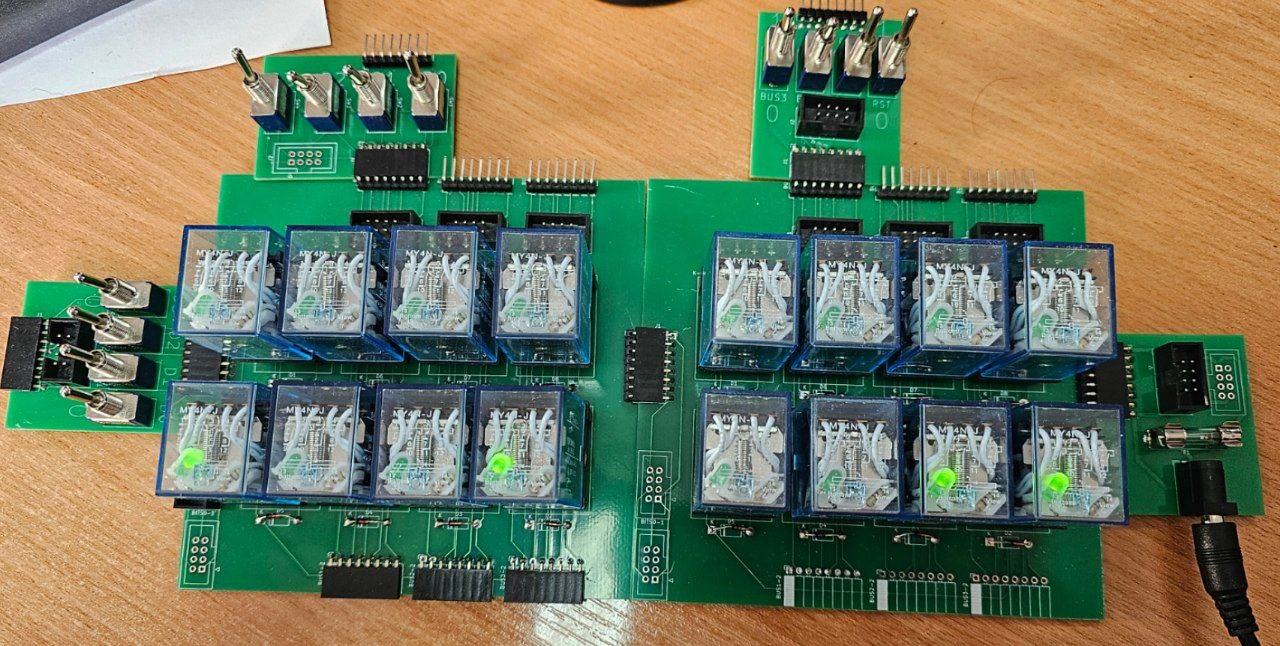
\includegraphics[width=0.5\columnwidth]{photo/8bit_register.jpg}

\begin{enumerate}
    \item Отключите все управляющие сигналы.
    \item Наберите входные данные $0011 1001$.
    \item Подключите тумблеры с данными к шине $1$, подав соответствующий управляющий сигнал.
    \item Отключите регистры от шины.
    \item Убедитесь, что восьмибитное значение сохранилось
    \item Подайте сигнал сброса на регистры.
    \item Убедитесь, что оба регистра обнулились.
\end{enumerate}

